\section{Popis jednotlivých součástek a důvody konkrétního tvaru}

Trezor má tvar krychle a~délku hrany má 128~mm, násobek šestnácti jsem zvolil kvůli jednoduché návaznosti na dřívka, %todo přidáme pár vět o dřívkách 
dřevěná dřívka s obdélníkovým průřezem 3x16~mm nebo 2x16~mm.
Protože je trezor vyroben z překližky o síle 4~mm, jsou jeho vnitřní rozměry o 4~mm na každé straně menší (takže 122~mm).

\paragraph{Geometrie západky}
\begin{wrapfigure}{R}[0.2\textwidth]{0.7\textwidth}
    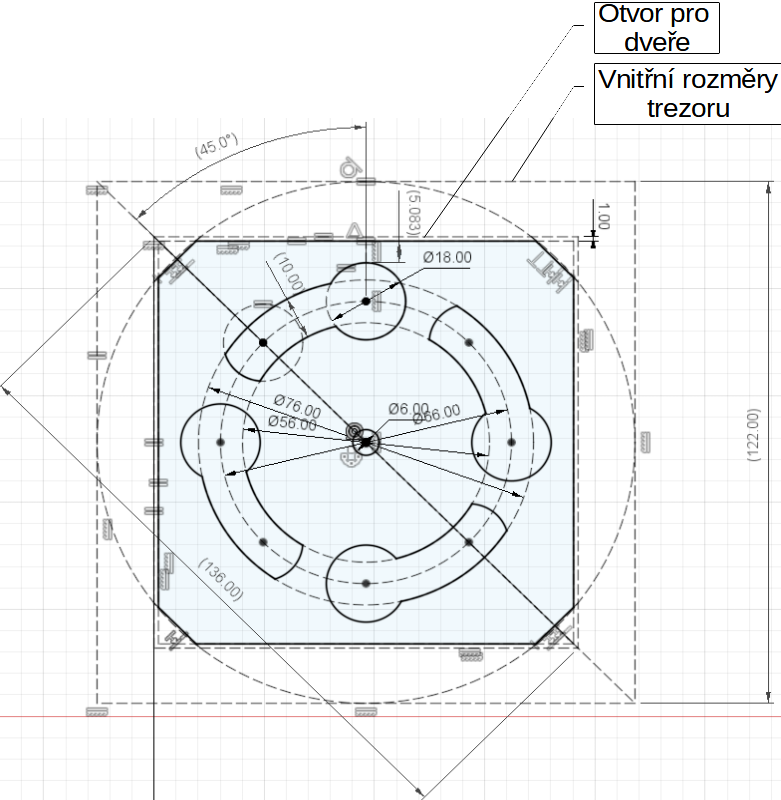
\includegraphics[width=0.7\textwidth]{kapitoly/obrazky/M3/geometrie_zapadky.png}
    \caption{náčrt západky} %todo čeho náčrt? 
    \label{fig:M3-geometrie-zapadky}
\end{wrapfigure} %todo zvážil bych obrázek centrovaný a obtékaný pouze nahoře a dole 

Protože se západka otáčí musí jí být zajištěn dostatek prostoru, zároveň však otvor pro dveře je lepší mít větší, protože se potom trezor dá použít pro větší objekty.
Z tohoto důvod jsou hrany západky definovány kružnicí o~průměru, délky vnitřní hrany trezoru. Západka má v~rozích sražení ze dvou důvodů. Za prvé aby byl otvor pro
dveře větší a~za~druhé aby namáhání působící v~západce působilo na větší délce.

\newpage

\paragraph{Distanční deska}

\begin{wrapfigure}{R}[0.2\textwidth]{0.7\textwidth}
    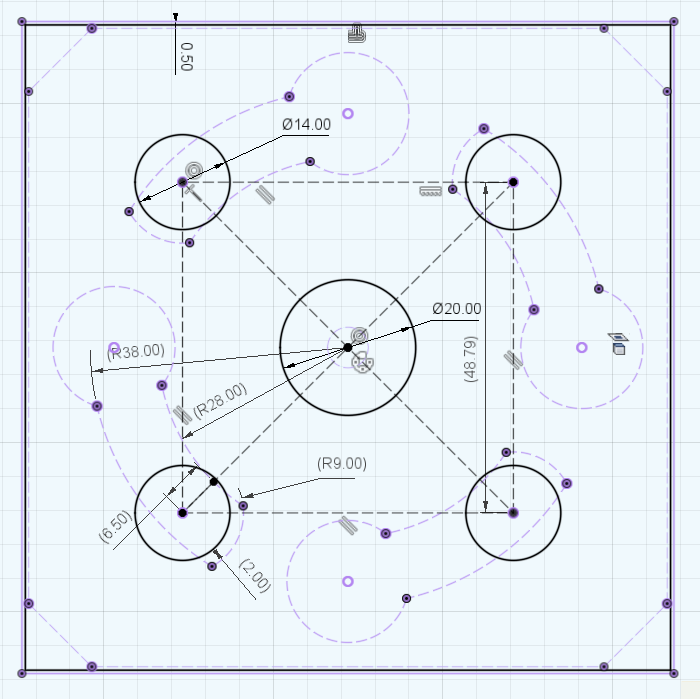
\includegraphics[width=0.7\textwidth]{kapitoly/obrazky/M3/distancka.png}
    \caption{náčrt Distanční desky}
    \label{fig:M3-distancka}
\end{wrapfigure}

Abi se západka dostala za desku přední stěny bedny trezoru je potřeba jí od přední stěny dveří posunout právě o tloušťku stěny. To zajišťuje jednoduchá čtvercová deska jen s~pěti otvory
pro průchod ovládacích kol.

\paragraph{Kámen} % jaksi mě nenapadl lepší název 
\begin{wrapfigure}{L}[0.2\textwidth]{0.7\textwidth}
    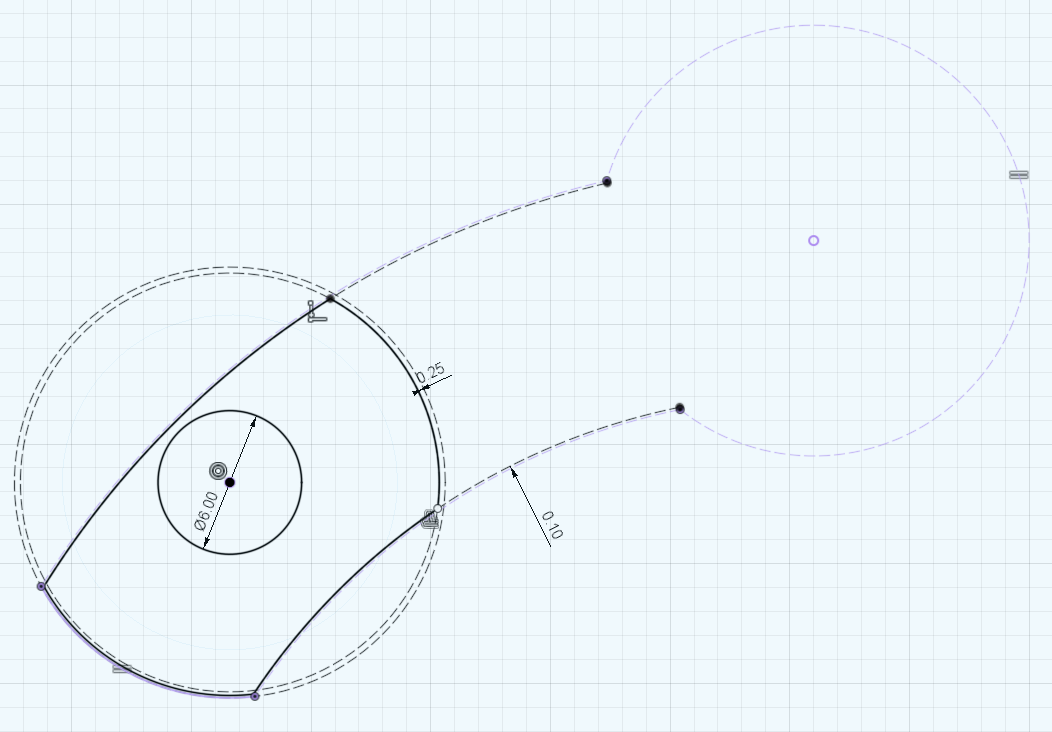
\includegraphics[width=0.7\textwidth]{kapitoly/obrazky/M3/kamen.png}
    \caption{náčrt kamene}
    \label{fig:M3-kamen}
\end{wrapfigure}

Kamen, který zajišťuje kód, má z~části tvar drážky, ve které jezdí, a~z~části kruh který se~muže otáčet v~kruhovém otvoru, na jedné staně drážky.
Uprostřed má~kruhoví otvor o~průměru 8mm pro kolík který kamenem otáčí.

\paragraph{Lepící distanční kroužek}

\begin{wrapfigure}{R}[0.2\textwidth]{0.7\textwidth}
    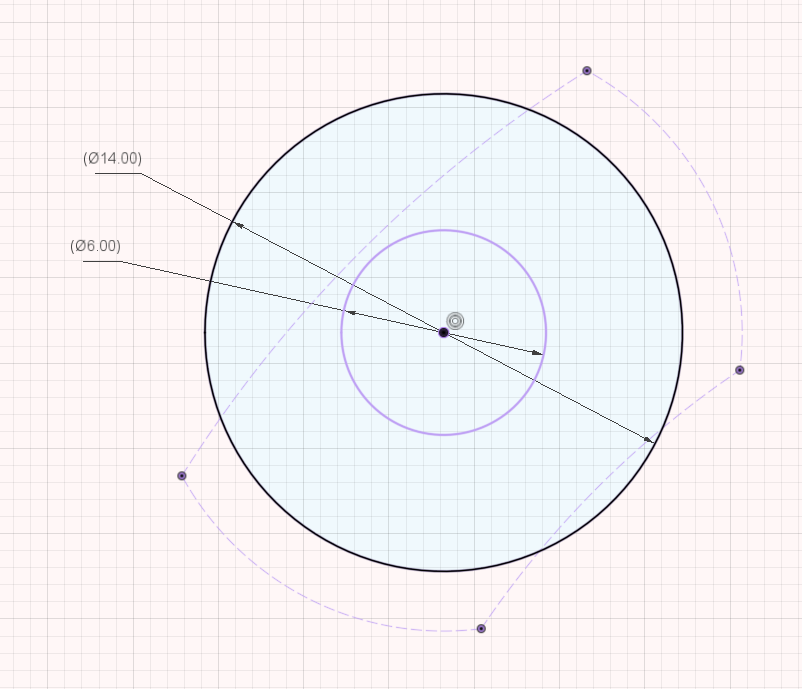
\includegraphics[width=0.7\textwidth]{kapitoly/obrazky/M3/lepici_distance.png}
    \caption{náčrt lepícího distančního kroužku}
    \label{fig:M3-lepici-distance}
\end{wrapfigure}

Tyto distanční kroužky jsou zde čistě z~technologického důvodu. Při lepení kolíku, totiž měli děti problém s~lepidlem, které jim zatékalo do~prostoru mezi kolíkem 
a~stěnou dveří čímž znemožňovalo otáčení kol. Proto jsem přidal tyto kroužky, do~kterých když zateče lepidlo tak~se nic neděje.

\newpage